\begin{homeworkProblem}[6]
    \begin{enumerate}
    \item \begin{multicols}{2}
    As seen in this graph of 6a, each initial condition produces a unique
    exponential mapping, however, all the mappings follow the same pattern and are
    unstable.
    $$
    x_{n+2} – 7x_{n+1} + 10x_n = 0
    $$

    \begin{figure}[H]
        \centering
        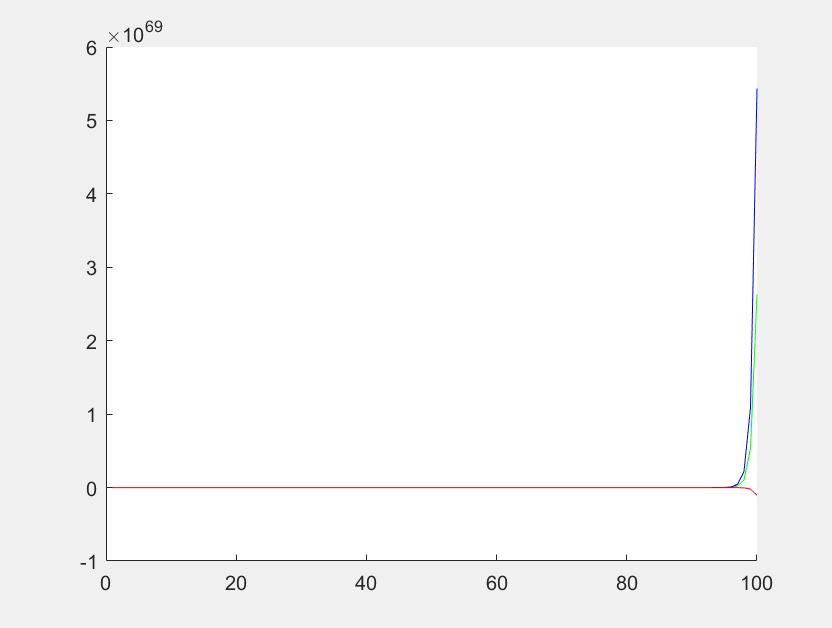
\includegraphics[scale=0.3]{fig/fig6(a).png}
    \end{figure}

    \end{multicols}

    \begin{listing}[htbp]
        \begin{tcolorbox}
        \begin{minted}{matlab}
    clear all
    eig1=5; eig2=2;
    x(1)=0;
    x(2)=1;
    x(3)=0.5;
    x(4)=-0.1;
    x(5)=2;
    x(6)=3;
    n=linspace(1,500);
    for k=1:2:6
        syms A B
        [solA,solB] = solve(
            A*eig1^x(k) + B*eig2^x(k) == x(k),
            A*eig1^x(k+1) + B*eig2^x(k+1) == x(k+1));
        n=[1:1:100];
        if k == 1
            hold on
            g=solA.*eig1.^n + solB.*eig2.^n;
            plot(n,g,'g')
        elseif k == 3
            hold on
            b=solA.*eig1.^n + solB.*eig2.^n;
            plot(n,b,'b')
        else
            hold on
            r=solA.*eig1.^n + solB.*eig2.^n;
            plot(n,solA.*eig1.^n + solB.*eig2.^n,'r')
        end
    end
        \end{minted}
        \end{tcolorbox}
    \end{listing}
    \pagebreak
    \begin{multicols}{2}
    (c). As seen in this graph of 6c, each initial condition produces a unique
    exponential mapping, however, all the mappings follow the same pattern and are
    unstable.
    $$
    x_{n+2} - \sigma_1 x_{n+1} + \sigma_2 x_n = 0
    $$

    \begin{figure}[H]
        \centering
        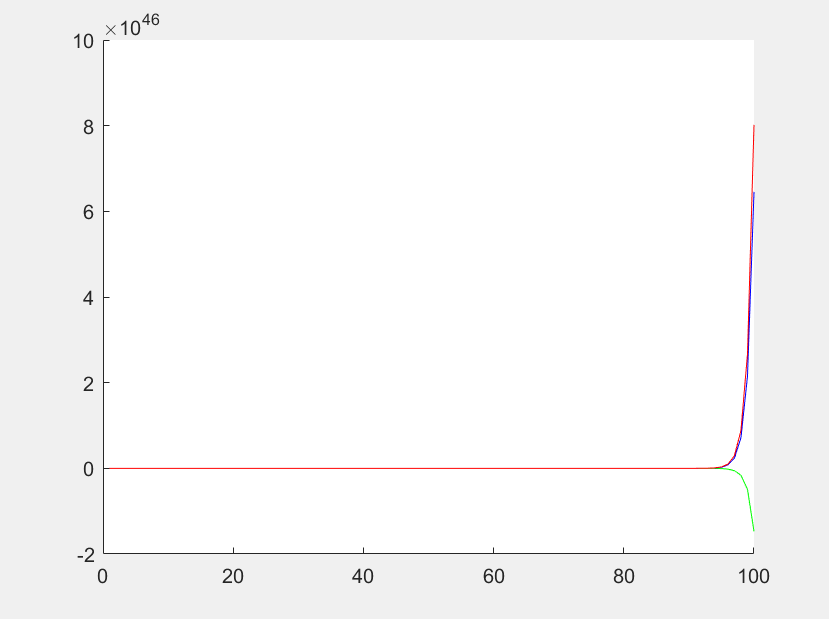
\includegraphics[scale=0.35]{fig/fig6(c).png}
    \end{figure}
    \end{multicols}
    \begin{listing}[htbp]
        \begin{tcolorbox}
        \begin{minted}{matlab}
    clear all
    s1= -1;
    s2= -2;
    beta= 3;
    eig1=(1/2)*(-s1+(sqrt(s1^2 -4*s2*beta)))
    eig2=(1/2)*(-s1-(sqrt(s1^2 -4*s2*beta)))
    x(1)=7;
    x(2)=1;
    x(3)=0.5;
    x(4)=-0.1;
    x(5)=2;
    x(6)=3;
    n=linspace(1,500);
    for k=1:2:6
        syms A B
        [solA,solB] = solve(
            A*eig1^x(k) + B*eig2^x(k) == x(k),
            A*eig1^x(k+1) + B*eig2^x(k+1) == x(k+1));
        n=[1:1:100];
        if k == 1
            hold on
            g=solA.*eig1.^n + solB.*eig2.^n;
            plot(n,g,'g')
        elseif k == 3
            hold on
            b=solA.*eig1.^n + solB.*eig2.^n;
            plot(n,b,'b')
        else
            hold on
            r=solA.*eig1.^n + solB.*eig2.^n;
            plot(n,solA.*eig1.^n + solB.*eig2.^n,'r')
        end
    end
        \end{minted}
        \end{tcolorbox}
    \end{listing}
    \pagebreak
    \addtocounter{enumi}{4}

    \item \begin{multicols}{2}
    As seen in this graph of 6f, each initial condition produces a unique
    oscillating mapping, however, all the mappings follow the same pattern and are
    unstable.
    $$
    x_{n+2} – \frac{5}{4}x_{n+1} + \frac{11}{8}x_n = 0
    $$

    \begin{figure}[H]
        \centering
        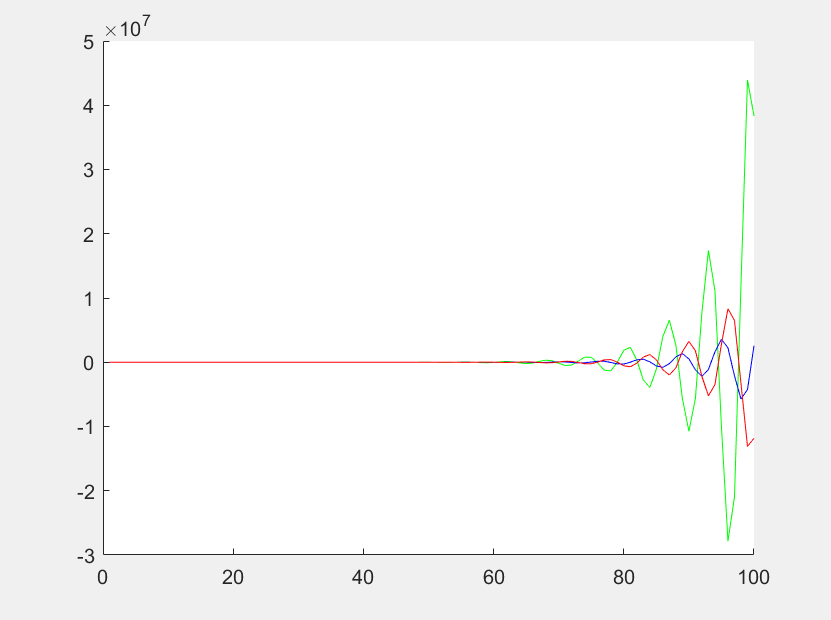
\includegraphics[scale=0.35]{fig/fig6(f).png}
    \end{figure}
    \end{multicols}

    \begin{listing}[htbp]
        \begin{tcolorbox}
        \begin{minted}{matlab}
    clear all
    eig1=(1/2)*(1.25+sqrt(1.5625-5.5))
    eig2=(1/2)*(1.25-sqrt(1.5625-5.5))
    x(1)=7;
    x(2)=1;
    x(3)=0.5;
    x(4)=-0.1;
    x(5)=2;
    x(6)=3;
    n=linspace(1,500);

    for k=1:2:6
        syms A B
        [solA,solB] = solve(
            A*eig1^x(k) + B*eig2^x(k) == x(k),
            A*eig1^x(k+1) + B*eig2^x(k+1) == x(k+1));
        n=[1:1:100];
        if k == 1
            hold on
            g=solA.*eig1.^n + solB.*eig2.^n;
            plot(n,g,'g')
        elseif k == 3
            hold on
            b=solA.*eig1.^n + solB.*eig2.^n;
            plot(n,b,'b')
        else
            hold on
            r=solA.*eig1.^n + solB.*eig2.^n;
            plot(n,solA.*eig1.^n + solB.*eig2.^n,'r')
        end
    end
        \end{minted}
        \end{tcolorbox}
    \end{listing}
    \end{enumerate}
    \end{homeworkProblem}